\documentclass[a4paper,12pt]{report}

\usepackage[T1]{fontenc}
\usepackage[english]{babel}
\usepackage{geometry}
\usepackage{graphicx}
\usepackage{amsmath, amssymb}
\usepackage{array}
\usepackage{booktabs}
\usepackage{hyperref}
\usepackage{float}
\usepackage{rotating}


\geometry{margin=2.5cm}

\begin{document}
\title{
    \textbf{Contract Central}\\
    Technical Documentation
}

\makeatletter
\def\@author{
    M1 Software Development \& Big Data -- ISEN Toulon\\
    \textbf{Academic Year:} 2024--2025\\
    \textbf{Team Members:}\\
    Capucine Debailleul (Project Manager)\\
    Alexis Dutaud\\
    Fabio Sintoni\\
    Larry Jason Tueno
}
\makeatother


\date{Supervised by Thomas Dandelot and Tony Varnier}

\maketitle
\tableofcontents
\newpage
 %%%%%%%%%%%%%%%%%%%%%%%%%%
%% Add your chapters here %%
 %%%%%%%%%%%%%%%%%%%%%%%%%%
\chapter{Introduction}

This project is a web application composed of several interconnected microservices. The goal is to provide users with access to their documents, automated analysis of their content, and an intuitive interface.

\section{Communication}
Microservices communicate through \textbf{Google Pub/Sub}, using structured messages.

\section{Frontend}
The frontend (built with Flutter) interacts with the main backend API. It provides:
\begin{itemize}
    \item user account management,
    \item document upload,
    \item visualization of document analysis results.
\end{itemize}
\chapter{Microservice NestBackend}

\section{Overview}
\textbf{NestBackend} is the main backend service of the system. It integrates several key modules.

\section{Main Features}
\begin{itemize}
    \item \textbf{Authentication} using Firebase Auth
    \item \textbf{Firebase} in a GCP Cloud Storage bucket
    \item \textbf{VertexAI} with Gemini pro 1.5
    \item \textbf{Pub/Sub} messaging to communicate with DocAnalysis
    \item \textbf{Dashboard} for user to manage their documents
    \item \textbf{User} for user management
\end{itemize}

\section{Dependencies}

This section outlines the dependencies required for the backend service, categorized into service dependencies and development dependencies. Each dependency is listed with its purpose to provide clarity on its role within the project.
The backend service is built using the NestJS framework and integrates with various Google Cloud services, including Firebase and Vertex AI. The dependencies are managed using npm and are specified in the \texttt{package.json} file.

\subsection{Service Dependencies}

\begin{tabular}{>{\bfseries}l l}
\toprule
Package & Purpose \\
\midrule
@google-cloud/aiplatform & Vertex AI SDK for ML requests \\
@google-cloud/pubsub & Google Pub/Sub messaging system \\
@google-cloud/secret-manager & Secure storage and access to secrets \\
@google-cloud/vertexai & Vertex AI high-level client (simplified) \\
@nestjs/common & NestJS decorators and helpers \\
@nestjs/config & Environment configuration management \\
@nestjs/core & NestJS core engine \\
@nestjs/microservices & Microservice architecture support \\
@nestjs/platform-express & Express integration with NestJS \\
@nestjs/swagger & OpenAPI documentation generator \\
@types/multer & Type definitions for multer \\
class-transformer & DTO class serialization/deserialization \\
class-validator & DTO input validation \\
firebase-admin & Firebase Admin SDK (Auth, Firestore, GCS) \\
multer & Middleware for file uploads \\
nestjs-pino & Structured logging with Pino in NestJS \\
pino & High-performance JSON logger \\
reflect-metadata & Required for decorators/reflection \\
rxjs & Reactive programming and Observables \\
swagger-ui-express & Swagger UI middleware for Express \\
\bottomrule
\end{tabular}

\subsection{Dev Dependencies}

\begin{tabular}{>{\bfseries}l l}
\toprule
Package & Purpose \\
\midrule
@nestjs/cli & NestJS project scaffolding and commands \\
@nestjs/schematics & Code generation templates for NestJS \\
@nestjs/testing & Utilities for unit and integration tests \\
@types/express & Type definitions for Express.js \\
@types/jest & Type definitions for Jest \\
@types/node & Type definitions for Node.js \\
@types/supertest & Type definitions for Supertest \\
@typescript-eslint/eslint-plugin & ESLint rules for TypeScript \\
@typescript-eslint/parser & Parser to enable ESLint for TS \\
eslint & Linter for code quality \\
eslint-config-prettier & Disables rules that conflict with Prettier \\
eslint-plugin-prettier & Integrates Prettier into ESLint \\
jest & Testing framework \\
prettier & Code formatter \\
source-map-support & Stack trace source map translation \\
supertest & HTTP assertions for integration tests \\
ts-jest & Jest preprocessor for TypeScript \\
ts-loader & TypeScript loader for Webpack \\
ts-node & Run TypeScript files directly \\
tsconfig-paths & Support for path aliases in tsconfig \\
typescript & TypeScript compiler \\
\bottomrule
\end{tabular}
\section{User Module}

\subsection*{Overview}

The \textbf{UserModule} manages user-specific metadata and preferences that are not handled by Firebase Auth. It stores and retrieves information such as first name, last name, birthdate, and contact data using Firestore.

\subsection*{Responsibilities}

\begin{itemize}
    \item Create and update user profile information in Firestore.
    \item Retrieve authenticated user metadata (from Firebase Auth).
    \item Provide a minimal contact endpoint for support messages (placeholder).
\end{itemize}

\subsection*{Dependencies}

\begin{itemize}
    \item \texttt{Firestore} - Used to store extended user info.
    \item \texttt{AuthService} - Used to fetch Firebase Auth metadata (e.g., display name, email).
\end{itemize}

\subsection*{Key Service Methods}

\begin{itemize}
    \item \texttt{createUserInfo(uid, dto)}: Creates a Firestore document with full name and email pulled from Firebase Auth.
    \item \texttt{updateUserInfo(uid, dto)}: Updates the user info with merge semantics and a timestamp.
    \item \texttt{getUserInfo(uid)}: Returns user info from Firestore, or \texttt{null} if not found.
\end{itemize}

\subsection*{Exposed Routes}

\subsubsection*{POST /user/me}

\begin{tabular}{>{\bfseries}l l}
\toprule
Method & POST \\
Route & /user/me \\
Auth required & Yes \\
Status codes & 201 Created, 400 Bad Request, 401 Unauthorized \\
\bottomrule
\end{tabular}

\textbf{Description:} Creates the Firestore user profile based on the authenticated user's UID and metadata from Firebase Auth.

\vspace{1em}
\textbf{Payload Example:}
\begin{verbatim}
{
  "birthdate": "2000-01-01"
}
\end{verbatim}

\subsubsection*{PATCH /user/me}

\begin{tabular}{>{\bfseries}l l}
\toprule
Method & PATCH \\
Route & /user/me \\
Auth required & Yes \\
Status codes & 200 OK, 400 Bad Request, 401 Unauthorized \\
\bottomrule
\end{tabular}

\textbf{Description:} Updates user information in Firestore. Uses \texttt{merge: true} semantics to preserve existing fields.

\vspace{1em}
\textbf{Payload Example:}
\begin{verbatim}
{
  "firstname": "Jane",
  "lastname": "Smith",
  "email": "jane@example.com"
}
\end{verbatim}

\subsubsection*{POST /user/contact}

\begin{tabular}{>{\bfseries}l l}
\toprule
Method & POST \\
Route & /user/contact \\
Auth required & No \\
Status codes & 200 OK (placeholder) \\
\bottomrule
\end{tabular}

\textbf{Description:} Endpoint for users to contact admin/support. Currently a stub (to be implemented).

\vspace{1em}
\textbf{Payload Example:}
\begin{verbatim}
{
  "email": "user@example.com",
  "message": "I need help with..."
}
\end{verbatim}

\subsection*{Testing}

Unit tests validate:

\begin{itemize}
    \item Creation of user info from Firebase metadata.
    \item Updating user info with merge semantics.
    \item Retrieval of user data (existing and non-existing cases).
\end{itemize}

Mocks are used for:

\begin{itemize}
    \item \texttt{AuthService.getUserByUid()}
    \item Firestore collection, doc, set, and get operations
\end{itemize}

\section{Firebase Module}

\subsection*{Overview}

The \textbf{FirebaseModule} is a global dynamic module that initializes the Firebase Admin SDK and exposes key Firebase services throughout the application. It centralizes configuration and ensures consistent access to Firebase features like Firestore, Auth, and Cloud Storage.

\subsection*{Responsibilities}

\begin{itemize}
    \item Initialize Firebase Admin with default credentials.
    \item Provide access to:
        \begin{itemize}
            \item Firestore (NoSQL database)
            \item Firebase Authentication
            \item Cloud Storage bucket
        \end{itemize}
    \item Export these providers globally to be used by other modules (e.g., Auth, Files, Dashboard).
\end{itemize}

\subsection*{Dynamic Initialization}

\textbf{FirebaseModule.forRoot()} returns a \texttt{DynamicModule} configured with the following providers:

\begin{itemize}
    \item \textbf{FIREBASE\_APP} - Firebase application instance
    \item \textbf{FIRESTORE} - Firestore database instance
    \item \textbf{FIREBASE\_AUTH} - Firebase authentication handler
    \item \textbf{FIREBASE\_BUCKET} - Google Cloud Storage bucket handler
\end{itemize}

These tokens are injected via NestJS's dependency injection system.

\subsection*{Global Scope}

The module is marked with \texttt{@Global()} so it only needs to be imported once and is accessible throughout the entire application without re-importing in each feature module.

\subsection*{Testing}

A dedicated unit test verifies that:
\begin{itemize}
    \item All Firebase services are correctly provided via dependency tokens.
    \item The module exports all necessary services.
\end{itemize}

Mocked Firebase services are used in unit tests to avoid external dependency on Firebase during test execution.

\subsection*{Configuration}

\begin{itemize}
    \item \textbf{Project ID:} \texttt{contract-central-c710c}
    \item \textbf{Storage Bucket:} \texttt{contract-central-c710c.firebasestorage.app}
    \item \textbf{Credential:} Application Default Credential
\end{itemize}

\section{File Module}

\subsection*{Overview}

The \textbf{FileModule} manages all user file operations including upload, retrieval, deletion, and temporary storage. It integrates Google Cloud Storage via Firebase and uses Pub/Sub to notify other microservices of file-related events.

\subsection*{Responsibilities}

\begin{itemize}
    \item Upload and store user files under structured paths in GCS.
    \item Generate temporary signed URLs for accessing files.
    \item Delete specific or all files for a user.
    \item Notify other services of file upload and deletion via Pub/Sub.
\end{itemize}

\subsection*{Dependencies}

\begin{itemize}
    \item \texttt{@google-cloud/storage} - for GCS bucket access.
    \item \texttt{FirebaseModule} - to inject the GCS bucket.
    \item \texttt{PubSubService} - to publish \texttt{file-upload} and \texttt{file-delete} events.
\end{itemize}

\subsection*{Key Service Methods}

\begin{itemize}
    \item \texttt{uploadFile(uid, file, dto)} - Uploads a categorized file and emits Pub/Sub event.
    \item \texttt{getFileUrl(uid, fileName)} - Returns a temporary signed URL for a user file.
    \item \texttt{getUserFiles(uid)} - Lists all files uploaded by the user.
    \item \texttt{deleteFile(uid, fname, category)} - Deletes a file and emits a Pub/Sub event.
    \item \texttt{deleteAllUserFiles(uid)} - Deletes all user files and emits a single Pub/Sub event.
    \item \texttt{uploadTmpImage(uid, file, dto)} - Special-purpose method to upload temporary images.
    \item \texttt{deleteTempFile(fpath)} - Deletes a temporary file if it exists.
\end{itemize}

\subsection*{Exposed Routes}

\subsubsection*{POST /files/upload}

\begin{tabular}{>{\bfseries}l l}
\toprule
Method & POST \\
Route & /files/upload \\
Auth required & Yes \\
Consumes & multipart/form-data \\
\bottomrule
\end{tabular}

\vspace{1em}
\textbf{Form fields:}
\begin{itemize}
    \item \texttt{file}: PDF file to upload
    \item \texttt{category}: required category label (e.g., \texttt{HEALTH}, \texttt{EMPLOYMENT})
\end{itemize}

\subsubsection*{GET /files/:fileName}

Returns a temporary signed URL for the requested file.

\subsubsection*{GET /files}

Returns a list of all files uploaded by the authenticated user.

\subsubsection*{DELETE /files/:category/:fileName}

Deletes a specific file in a category and emits a \texttt{file-delete} event.

\subsubsection*{DELETE /files}

Deletes all files for the user and emits a single \texttt{file-delete} event.

\subsection*{Error Handling}

\begin{itemize}
    \item \textbf{400 Bad Request} - Invalid or missing category.
    \item \textbf{404 Not Found} - Requested file does not exist.
    \item \textbf{500 Internal Server Error} - Upload/delete/signing failures.
\end{itemize}

\subsection*{Testing}

Unit tests validate:

\begin{itemize}
    \item File upload with event publishing.
    \item Temporary signed URL generation.
    \item Accurate file listing.
    \item Conditional deletion (specific or all files).
    \item Handling of missing files and errors.
\end{itemize}

Mocks are used for:

\begin{itemize}
    \item GCS Bucket and File objects.
    \item Pub/Sub message publishing.
\end{itemize}

\section{VertexAI Module}

\subsection*{Overview}

The \textbf{VertexAI Module} integrates the Google Cloud Vertex AI API into the backend using the \texttt{@google-cloud/vertexai} client. It handles AI-driven reasoning and recommendation tasks by interacting with Gemini 1.5 Pro.

\subsection*{Responsibilities}

\begin{itemize}
    \item Load a generative model (Gemini 1.5 Pro) via the Vertex AI SDK.
    \item Process user prompts and file references (PDF, images).
    \item Generate structured reasoning and actionable recommendations.
    \item Log AI interactions to Firestore for traceability.
\end{itemize}

\subsection*{Workflow Summary}

The method \texttt{generateTextContent} executes two chained LLM calls:

\begin{enumerate}
    \item \textbf{Structured reasoning generation} based on:
    \begin{itemize}
        \item User metadata (\texttt{firstname}, \texttt{lastname}, etc.)
        \item Attached files from Firebase Storage
        \item Custom domain-specific reasoning prompt
    \end{itemize}
    \item \textbf{Final decision generation} based on the AI's reasoning output.
\end{enumerate}

Results are logged in Firestore under the \texttt{logs/\{uid\}/ai\_interactions} collection with full metadata.

\subsection*{Prompt Logic}

\begin{itemize}
    \item Prompts are composed dynamically using the user's identity and structured business rules.
    \item \textbf{Reasoning Prompt:} guides the model to extract risk analysis and contract redundancies.
    \item \textbf{Final Decision Prompt:} asks the model to produce an actionable summary.
    \item All file attachments are referenced using GCS URIs (e.g., \texttt{gs://bucket/path}).
\end{itemize}

\subsection*{Key Method: \texttt{generateTextContent}}

\begin{itemize}
    \item \textbf{Inputs:} user ID, prompt string, list of Firebase Storage URLs, user metadata.
    \item \textbf{Output:} response object from Vertex AI's LLM (Gemini 1.5 Pro).
    \item \textbf{Side-effects:}
    \begin{itemize}
        \item AI interaction logs written to Firestore.
        \item Token usage, model version, and response IDs tracked.
    \end{itemize}
\end{itemize}

\subsection*{Firestore Logging Structure}

Each interaction creates or updates a Firestore document with:

\begin{itemize}
    \item \texttt{prompt}, \texttt{reasoning}, \texttt{finalDecision}
    \item \texttt{vertexResponse} and \texttt{finalVertexResponse} metadata
    \item \texttt{createdAt}, \texttt{deletedAt}
\end{itemize}

\subsection*{Error Handling}

\begin{itemize}
    \item If reasoning or decision generation fails, the error is logged and rethrown.
    \item GCS URI generation fallback uses MIME type detection to support different file types.
\end{itemize}

\subsection*{Testing}

Unit tests validate:

\begin{itemize}
    \item Proper generation of both reasoning and final decision via mocked LLM.
    \item Firestore logs are created and updated accordingly.
    \item Token usage, model version, and response IDs are extracted correctly.
\end{itemize}

Mocks are used for:

\begin{itemize}
    \item VertexAI client and model generation responses.
    \item Firestore document creation and update.
\end{itemize}

\section{Dashboard Module}

\subsection*{Overview}

The \textbf{Dashboard} module provides a synthetic view of a user's activity and data. It aggregates file statistics and coverage request history from Firestore and returns a structured dashboard summary.

\subsection*{Responsibilities}

\begin{itemize}
    \item Aggregate file statistics per user from Cloud Storage.
    \item Count and classify AI coverage requests (pending / completed).
    \item Return a structured summary to the frontend.
\end{itemize}

\subsection*{Dependencies}

\begin{itemize}
    \item \texttt{FileService} - for retrieving user files from storage.
    \item \texttt{Firestore} - for querying the \texttt{coverage\_requests} collection.
    \item \texttt{@nestjs/common} - for DI and controller structure.
\end{itemize}

\subsection*{Main Service Method}

\begin{itemize}
    \item \textbf{buildDashboard(uid: string)}: builds and returns a \texttt{DashboardDto} object containing:
    \begin{itemize}
        \item Total number of user files
        \item Breakdown of files by category
        \item Coverage requests (pending and completed)
        \item Recent request history (max 20)
    \end{itemize}
\end{itemize}

\subsection*{Resilience Handling}

If the required Firestore index is missing, a partial dashboard is returned with empty coverage history. This ensures continued availability even when Firestore is misconfigured.

\subsection*{Exposed Route}

\subsubsection*{GET /dashboard}

\begin{tabular}{>{\bfseries}l l}
\toprule
Method & GET \\
Route & /dashboard \\
Auth required & Yes (via Firebase ID token) \\
Status codes & 200 OK, 500 Internal Server Error \\
\bottomrule
\end{tabular}

\vspace{1em}
\textbf{Headers:}
\begin{verbatim}
Authorization: Bearer <ID_TOKEN>
\end{verbatim}

\vspace{1em}
\textbf{Success Response:}
\begin{verbatim}
Status: 200 OK
{
  "totalFiles": 3,
  "filesByCategory": {
    "health": 1,
    "employment": 2
  },
  "pendingCoverageRequests": 1,
  "completedCoverageRequests": 4,
  "coverageHistory": [
    {
      "requestId": "abc123",
      "prompt": "What is my health coverage?",
      "status": "done",
      "response": "...",
      "updatedAt": 1716170000000
    }
  ]
}
\end{verbatim}

\vspace{1em}
\textbf{Error Responses:}
\begin{itemize}
    \item \textbf{500 Internal Server Error} - Firestore failure or exception.
\end{itemize}

\section{PubSub Module}

\subsection*{Overview}

The \textbf{PubSubModule} encapsulates the Google Cloud Pub/Sub integration used by the application to handle asynchronous communication between microservices. It publishes and subscribes to various event topics related to files and AI coverage analysis.

\subsection*{Responsibilities}

\begin{itemize}
    \item Publish events to specific Pub/Sub topics.
    \item Subscribe to the \texttt{coverage-response-sub} subscription.
    \item Update Firestore with AI coverage results upon message reception.
\end{itemize}

\subsection*{Topics Used}

\begin{itemize}
    \item \textbf{coverage-query} - Trigger coverage analysis requests.
    \item \textbf{coverage-response} - Receives responses from the AI service.
    \item \textbf{file-upload} - Event triggered when a file is uploaded.
    \item \textbf{file-delete} - Event triggered when a file is deleted.
\end{itemize}

\subsection*{Key Methods}

\begin{itemize}
    \item \texttt{publishMessage(topicName: string, data: object)} \\
    Publishes a JSON-encoded message to the specified Pub/Sub topic.

    \item \texttt{subscribeToCoverageResponse()} \\
    Subscribes to \texttt{coverage-response-sub} and processes AI results to update the Firestore \texttt{coverage\_requests} collection.
\end{itemize}

\subsection*{Error Handling}

If a received message is missing expected fields (\texttt{request\_id}, \texttt{user\_uuid}, or \texttt{response}), the message is rejected with \texttt{nack()}. Other exceptions are logged and also result in a negative acknowledgment.

\subsection*{Lifecycle Hook}

The service implements \texttt{OnModuleInit} and only subscribes to incoming Pub/Sub messages if the environment is not \texttt{"test"}. This allows for isolated unit testing without background consumers.

\subsection*{Testing}

Unit tests verify:
\begin{itemize}
    \item That messages are published correctly with expected parameters.
    \item That the \texttt{subscribeToCoverageResponse} method is invoked on module initialization (except in test mode).
    \item That Firestore is updated when a message is handled successfully.
\end{itemize}

Mocks are used for:
\begin{itemize}
    \item Pub/Sub client, topics and subscriptions.
    \item Firestore client and document operations.
\end{itemize}

\section{VertexAI Module}

\subsection*{Overview}

The \textbf{VertexAI Module} integrates the Google Cloud Vertex AI API into the backend using the \texttt{@google-cloud/vertexai} client. It handles AI-driven reasoning and recommendation tasks by interacting with Gemini 1.5 Pro.

\subsection*{Responsibilities}

\begin{itemize}
    \item Load a generative model (Gemini 1.5 Pro) via the Vertex AI SDK.
    \item Process user prompts and file references (PDF, images).
    \item Generate structured reasoning and actionable recommendations.
    \item Log AI interactions to Firestore for traceability.
\end{itemize}

\subsection*{Workflow Summary}

The method \texttt{generateTextContent} executes two chained LLM calls:

\begin{enumerate}
    \item \textbf{Structured reasoning generation} based on:
    \begin{itemize}
        \item User metadata (\texttt{firstname}, \texttt{lastname}, etc.)
        \item Attached files from Firebase Storage
        \item Custom domain-specific reasoning prompt
    \end{itemize}
    \item \textbf{Final decision generation} based on the AI's reasoning output.
\end{enumerate}

Results are logged in Firestore under the \texttt{logs/\{uid\}/ai\_interactions} collection with full metadata.

\subsection*{Prompt Logic}

\begin{itemize}
    \item Prompts are composed dynamically using the user's identity and structured business rules.
    \item \textbf{Reasoning Prompt:} guides the model to extract risk analysis and contract redundancies.
    \item \textbf{Final Decision Prompt:} asks the model to produce an actionable summary.
    \item All file attachments are referenced using GCS URIs (e.g., \texttt{gs://bucket/path}).
\end{itemize}

\subsection*{Key Method: \texttt{generateTextContent}}

\begin{itemize}
    \item \textbf{Inputs:} user ID, prompt string, list of Firebase Storage URLs, user metadata.
    \item \textbf{Output:} response object from Vertex AI's LLM (Gemini 1.5 Pro).
    \item \textbf{Side-effects:}
    \begin{itemize}
        \item AI interaction logs written to Firestore.
        \item Token usage, model version, and response IDs tracked.
    \end{itemize}
\end{itemize}

\subsection*{Firestore Logging Structure}

Each interaction creates or updates a Firestore document with:

\begin{itemize}
    \item \texttt{prompt}, \texttt{reasoning}, \texttt{finalDecision}
    \item \texttt{vertexResponse} and \texttt{finalVertexResponse} metadata
    \item \texttt{createdAt}, \texttt{deletedAt}
\end{itemize}

\subsection*{Error Handling}

\begin{itemize}
    \item If reasoning or decision generation fails, the error is logged and rethrown.
    \item GCS URI generation fallback uses MIME type detection to support different file types.
\end{itemize}

\subsection*{Testing}

Unit tests validate:

\begin{itemize}
    \item Proper generation of both reasoning and final decision via mocked LLM.
    \item Firestore logs are created and updated accordingly.
    \item Token usage, model version, and response IDs are extracted correctly.
\end{itemize}

Mocks are used for:

\begin{itemize}
    \item VertexAI client and model generation responses.
    \item Firestore document creation and update.
\end{itemize}

\section{Auth Module}

\subsection*{Overview}

The \textbf{Auth} module handles user creation and authentication token validation using the Firebase Admin SDK. It provides a simple REST interface to register new users and verify existing sessions.

\subsection*{Responsibilities}

\begin{itemize}
    \item Creating new users via Firebase.
    \item Verifying ID tokens for secure API access.
    \item Fetching user information by UID.
\end{itemize}

\subsection*{Dependencies}

\begin{itemize}
    \item \texttt{firebase-admin} - for user management and token verification.
    \item \texttt{@nestjs/common} - core NestJS features.
    \item \texttt{class-validator} - request payload validation (via DTO).
\end{itemize}

\subsection*{Main Service Methods}

\begin{itemize}
    \item \textbf{create(dto: CreateUserDto)}: registers a user in Firebase.
    \item \textbf{checkToken(token: string)}: verifies a Firebase ID token.
    \item \textbf{getUserByUid(uid: string)}: fetches user data from Firebase.
\end{itemize}

\subsection*{Testing}

Unit tests are implemented with Jest and cover:
\begin{itemize}
    \item User creation with full name.
    \item Token verification.
    \item User retrieval by UID.
\end{itemize}

\subsection*{Exposed Route}

\subsubsection*{POST /auth/signin}

\begin{tabular}{>{\bfseries}l l}
\toprule
Method & POST \\
Route & /auth/signin \\
Auth required & No \\
Status codes & 201 Created, 400 Bad Request, 500 Internal Server Error \\
\bottomrule
\end{tabular}

\vspace{1em}
\textbf{Request Body:}
\begin{verbatim}
{
  "email": "john@example.com",
  "password": "securePass123",
  "firstname": "John",
  "lastname": "Doe"
}
\end{verbatim}

\vspace{1em}
\textbf{Success Response:}
\begin{verbatim}
Status: 201 Created
{
  "statusCode": 201,
  "message": "User created",
  "data": {
    "uid": "user123",
    ...
  }
}
\end{verbatim}

\vspace{1em}
\textbf{Error Responses:}
\begin{itemize}
    \item \textbf{400 Bad Request} - missing or invalid fields.
    \item \textbf{500 Internal Server Error} - Firebase failure or exception.
\end{itemize}

\subsection*{AI Interaction Sequence}

\begin{sidewaysfigure}
    \centering
    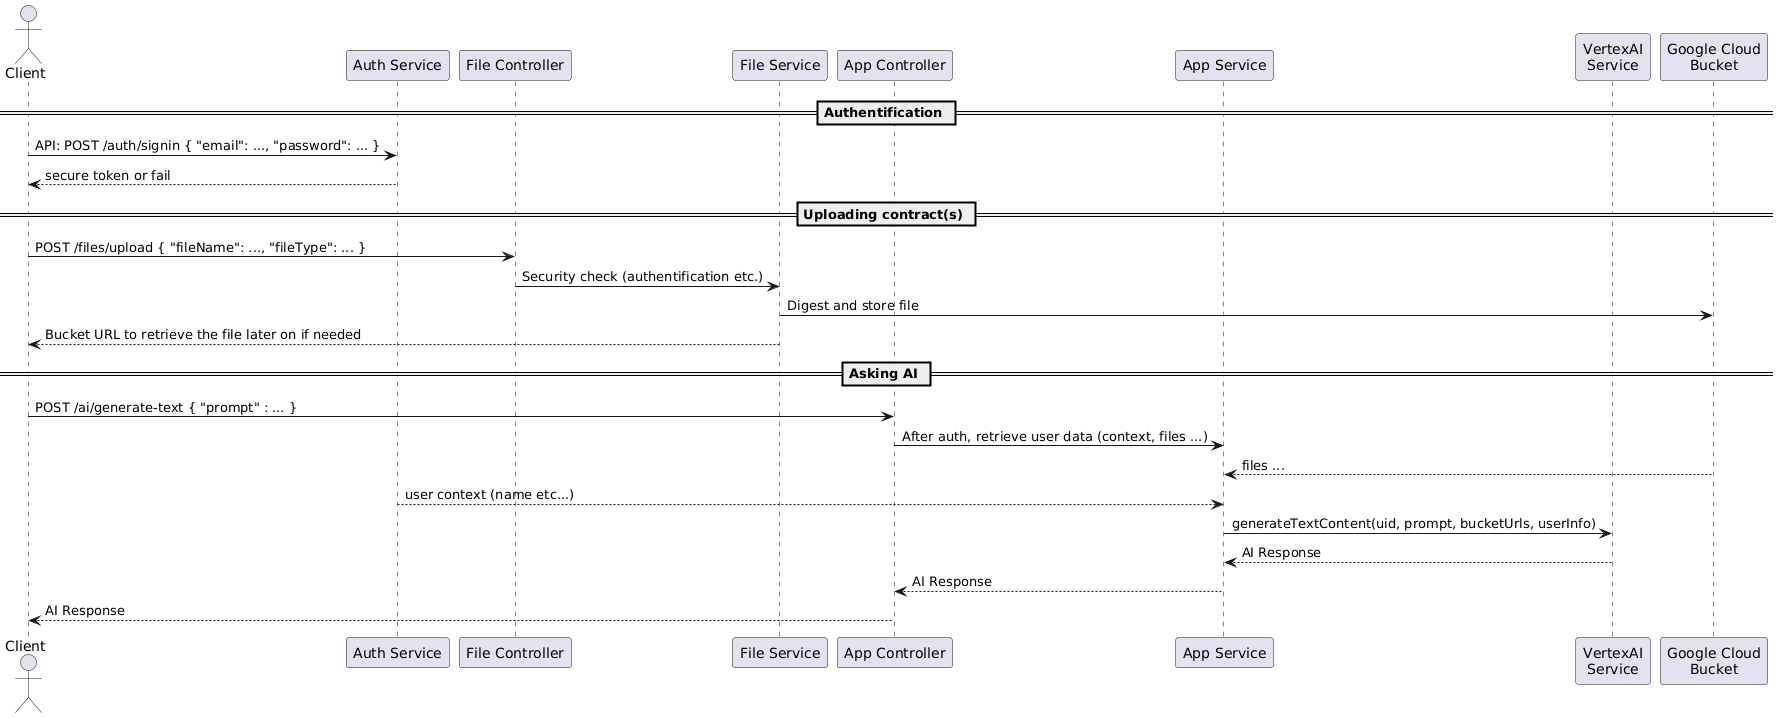
\includegraphics[width=\textheight]{nest/ai-sequence.png}
    \caption{Sequence diagram illustrating the AI processing flow}
    \label{fig:ai-sequence}
\end{sidewaysfigure}

\chapter{Microservice NestBackend}

\section{Overview}
\textbf{NestBackend} is the main backend service of the system. It integrates several key modules.

\section{Main Features}
\begin{itemize}
    \item \textbf{Authentication} using Firebase Auth
    \item \textbf{Firebase} in a GCP Cloud Storage bucket
    \item \textbf{VertexAI} with Gemini pro 1.5
    \item \textbf{Pub/Sub} messaging to communicate with DocAnalysis
    \item \textbf{Dashboard} for user to manage their documents
    \item \textbf{User} for user management
\end{itemize}

\section{Dependencies}

This section outlines the dependencies required for the backend service, categorized into service dependencies and development dependencies. Each dependency is listed with its purpose to provide clarity on its role within the project.
The backend service is built using the NestJS framework and integrates with various Google Cloud services, including Firebase and Vertex AI. The dependencies are managed using npm and are specified in the \texttt{package.json} file.

\subsection{Service Dependencies}

\begin{tabular}{>{\bfseries}l l}
\toprule
Package & Purpose \\
\midrule
@google-cloud/aiplatform & Vertex AI SDK for ML requests \\
@google-cloud/pubsub & Google Pub/Sub messaging system \\
@google-cloud/secret-manager & Secure storage and access to secrets \\
@google-cloud/vertexai & Vertex AI high-level client (simplified) \\
@nestjs/common & NestJS decorators and helpers \\
@nestjs/config & Environment configuration management \\
@nestjs/core & NestJS core engine \\
@nestjs/microservices & Microservice architecture support \\
@nestjs/platform-express & Express integration with NestJS \\
@nestjs/swagger & OpenAPI documentation generator \\
@types/multer & Type definitions for multer \\
class-transformer & DTO class serialization/deserialization \\
class-validator & DTO input validation \\
firebase-admin & Firebase Admin SDK (Auth, Firestore, GCS) \\
multer & Middleware for file uploads \\
nestjs-pino & Structured logging with Pino in NestJS \\
pino & High-performance JSON logger \\
reflect-metadata & Required for decorators/reflection \\
rxjs & Reactive programming and Observables \\
swagger-ui-express & Swagger UI middleware for Express \\
\bottomrule
\end{tabular}

\subsection{Dev Dependencies}

\begin{tabular}{>{\bfseries}l l}
\toprule
Package & Purpose \\
\midrule
@nestjs/cli & NestJS project scaffolding and commands \\
@nestjs/schematics & Code generation templates for NestJS \\
@nestjs/testing & Utilities for unit and integration tests \\
@types/express & Type definitions for Express.js \\
@types/jest & Type definitions for Jest \\
@types/node & Type definitions for Node.js \\
@types/supertest & Type definitions for Supertest \\
@typescript-eslint/eslint-plugin & ESLint rules for TypeScript \\
@typescript-eslint/parser & Parser to enable ESLint for TS \\
eslint & Linter for code quality \\
eslint-config-prettier & Disables rules that conflict with Prettier \\
eslint-plugin-prettier & Integrates Prettier into ESLint \\
jest & Testing framework \\
prettier & Code formatter \\
source-map-support & Stack trace source map translation \\
supertest & HTTP assertions for integration tests \\
ts-jest & Jest preprocessor for TypeScript \\
ts-loader & TypeScript loader for Webpack \\
ts-node & Run TypeScript files directly \\
tsconfig-paths & Support for path aliases in tsconfig \\
typescript & TypeScript compiler \\
\bottomrule
\end{tabular}
\section{User Module}

\subsection*{Overview}

The \textbf{UserModule} manages user-specific metadata and preferences that are not handled by Firebase Auth. It stores and retrieves information such as first name, last name, birthdate, and contact data using Firestore.

\subsection*{Responsibilities}

\begin{itemize}
    \item Create and update user profile information in Firestore.
    \item Retrieve authenticated user metadata (from Firebase Auth).
    \item Provide a minimal contact endpoint for support messages (placeholder).
\end{itemize}

\subsection*{Dependencies}

\begin{itemize}
    \item \texttt{Firestore} - Used to store extended user info.
    \item \texttt{AuthService} - Used to fetch Firebase Auth metadata (e.g., display name, email).
\end{itemize}

\subsection*{Key Service Methods}

\begin{itemize}
    \item \texttt{createUserInfo(uid, dto)}: Creates a Firestore document with full name and email pulled from Firebase Auth.
    \item \texttt{updateUserInfo(uid, dto)}: Updates the user info with merge semantics and a timestamp.
    \item \texttt{getUserInfo(uid)}: Returns user info from Firestore, or \texttt{null} if not found.
\end{itemize}

\subsection*{Exposed Routes}

\subsubsection*{POST /user/me}

\begin{tabular}{>{\bfseries}l l}
\toprule
Method & POST \\
Route & /user/me \\
Auth required & Yes \\
Status codes & 201 Created, 400 Bad Request, 401 Unauthorized \\
\bottomrule
\end{tabular}

\textbf{Description:} Creates the Firestore user profile based on the authenticated user's UID and metadata from Firebase Auth.

\vspace{1em}
\textbf{Payload Example:}
\begin{verbatim}
{
  "birthdate": "2000-01-01"
}
\end{verbatim}

\subsubsection*{PATCH /user/me}

\begin{tabular}{>{\bfseries}l l}
\toprule
Method & PATCH \\
Route & /user/me \\
Auth required & Yes \\
Status codes & 200 OK, 400 Bad Request, 401 Unauthorized \\
\bottomrule
\end{tabular}

\textbf{Description:} Updates user information in Firestore. Uses \texttt{merge: true} semantics to preserve existing fields.

\vspace{1em}
\textbf{Payload Example:}
\begin{verbatim}
{
  "firstname": "Jane",
  "lastname": "Smith",
  "email": "jane@example.com"
}
\end{verbatim}

\subsubsection*{POST /user/contact}

\begin{tabular}{>{\bfseries}l l}
\toprule
Method & POST \\
Route & /user/contact \\
Auth required & No \\
Status codes & 200 OK (placeholder) \\
\bottomrule
\end{tabular}

\textbf{Description:} Endpoint for users to contact admin/support. Currently a stub (to be implemented).

\vspace{1em}
\textbf{Payload Example:}
\begin{verbatim}
{
  "email": "user@example.com",
  "message": "I need help with..."
}
\end{verbatim}

\subsection*{Testing}

Unit tests validate:

\begin{itemize}
    \item Creation of user info from Firebase metadata.
    \item Updating user info with merge semantics.
    \item Retrieval of user data (existing and non-existing cases).
\end{itemize}

Mocks are used for:

\begin{itemize}
    \item \texttt{AuthService.getUserByUid()}
    \item Firestore collection, doc, set, and get operations
\end{itemize}

\section{Firebase Module}

\subsection*{Overview}

The \textbf{FirebaseModule} is a global dynamic module that initializes the Firebase Admin SDK and exposes key Firebase services throughout the application. It centralizes configuration and ensures consistent access to Firebase features like Firestore, Auth, and Cloud Storage.

\subsection*{Responsibilities}

\begin{itemize}
    \item Initialize Firebase Admin with default credentials.
    \item Provide access to:
        \begin{itemize}
            \item Firestore (NoSQL database)
            \item Firebase Authentication
            \item Cloud Storage bucket
        \end{itemize}
    \item Export these providers globally to be used by other modules (e.g., Auth, Files, Dashboard).
\end{itemize}

\subsection*{Dynamic Initialization}

\textbf{FirebaseModule.forRoot()} returns a \texttt{DynamicModule} configured with the following providers:

\begin{itemize}
    \item \textbf{FIREBASE\_APP} - Firebase application instance
    \item \textbf{FIRESTORE} - Firestore database instance
    \item \textbf{FIREBASE\_AUTH} - Firebase authentication handler
    \item \textbf{FIREBASE\_BUCKET} - Google Cloud Storage bucket handler
\end{itemize}

These tokens are injected via NestJS's dependency injection system.

\subsection*{Global Scope}

The module is marked with \texttt{@Global()} so it only needs to be imported once and is accessible throughout the entire application without re-importing in each feature module.

\subsection*{Testing}

A dedicated unit test verifies that:
\begin{itemize}
    \item All Firebase services are correctly provided via dependency tokens.
    \item The module exports all necessary services.
\end{itemize}

Mocked Firebase services are used in unit tests to avoid external dependency on Firebase during test execution.

\subsection*{Configuration}

\begin{itemize}
    \item \textbf{Project ID:} \texttt{contract-central-c710c}
    \item \textbf{Storage Bucket:} \texttt{contract-central-c710c.firebasestorage.app}
    \item \textbf{Credential:} Application Default Credential
\end{itemize}

\section{File Module}

\subsection*{Overview}

The \textbf{FileModule} manages all user file operations including upload, retrieval, deletion, and temporary storage. It integrates Google Cloud Storage via Firebase and uses Pub/Sub to notify other microservices of file-related events.

\subsection*{Responsibilities}

\begin{itemize}
    \item Upload and store user files under structured paths in GCS.
    \item Generate temporary signed URLs for accessing files.
    \item Delete specific or all files for a user.
    \item Notify other services of file upload and deletion via Pub/Sub.
\end{itemize}

\subsection*{Dependencies}

\begin{itemize}
    \item \texttt{@google-cloud/storage} - for GCS bucket access.
    \item \texttt{FirebaseModule} - to inject the GCS bucket.
    \item \texttt{PubSubService} - to publish \texttt{file-upload} and \texttt{file-delete} events.
\end{itemize}

\subsection*{Key Service Methods}

\begin{itemize}
    \item \texttt{uploadFile(uid, file, dto)} - Uploads a categorized file and emits Pub/Sub event.
    \item \texttt{getFileUrl(uid, fileName)} - Returns a temporary signed URL for a user file.
    \item \texttt{getUserFiles(uid)} - Lists all files uploaded by the user.
    \item \texttt{deleteFile(uid, fname, category)} - Deletes a file and emits a Pub/Sub event.
    \item \texttt{deleteAllUserFiles(uid)} - Deletes all user files and emits a single Pub/Sub event.
    \item \texttt{uploadTmpImage(uid, file, dto)} - Special-purpose method to upload temporary images.
    \item \texttt{deleteTempFile(fpath)} - Deletes a temporary file if it exists.
\end{itemize}

\subsection*{Exposed Routes}

\subsubsection*{POST /files/upload}

\begin{tabular}{>{\bfseries}l l}
\toprule
Method & POST \\
Route & /files/upload \\
Auth required & Yes \\
Consumes & multipart/form-data \\
\bottomrule
\end{tabular}

\vspace{1em}
\textbf{Form fields:}
\begin{itemize}
    \item \texttt{file}: PDF file to upload
    \item \texttt{category}: required category label (e.g., \texttt{HEALTH}, \texttt{EMPLOYMENT})
\end{itemize}

\subsubsection*{GET /files/:fileName}

Returns a temporary signed URL for the requested file.

\subsubsection*{GET /files}

Returns a list of all files uploaded by the authenticated user.

\subsubsection*{DELETE /files/:category/:fileName}

Deletes a specific file in a category and emits a \texttt{file-delete} event.

\subsubsection*{DELETE /files}

Deletes all files for the user and emits a single \texttt{file-delete} event.

\subsection*{Error Handling}

\begin{itemize}
    \item \textbf{400 Bad Request} - Invalid or missing category.
    \item \textbf{404 Not Found} - Requested file does not exist.
    \item \textbf{500 Internal Server Error} - Upload/delete/signing failures.
\end{itemize}

\subsection*{Testing}

Unit tests validate:

\begin{itemize}
    \item File upload with event publishing.
    \item Temporary signed URL generation.
    \item Accurate file listing.
    \item Conditional deletion (specific or all files).
    \item Handling of missing files and errors.
\end{itemize}

Mocks are used for:

\begin{itemize}
    \item GCS Bucket and File objects.
    \item Pub/Sub message publishing.
\end{itemize}

\section{VertexAI Module}

\subsection*{Overview}

The \textbf{VertexAI Module} integrates the Google Cloud Vertex AI API into the backend using the \texttt{@google-cloud/vertexai} client. It handles AI-driven reasoning and recommendation tasks by interacting with Gemini 1.5 Pro.

\subsection*{Responsibilities}

\begin{itemize}
    \item Load a generative model (Gemini 1.5 Pro) via the Vertex AI SDK.
    \item Process user prompts and file references (PDF, images).
    \item Generate structured reasoning and actionable recommendations.
    \item Log AI interactions to Firestore for traceability.
\end{itemize}

\subsection*{Workflow Summary}

The method \texttt{generateTextContent} executes two chained LLM calls:

\begin{enumerate}
    \item \textbf{Structured reasoning generation} based on:
    \begin{itemize}
        \item User metadata (\texttt{firstname}, \texttt{lastname}, etc.)
        \item Attached files from Firebase Storage
        \item Custom domain-specific reasoning prompt
    \end{itemize}
    \item \textbf{Final decision generation} based on the AI's reasoning output.
\end{enumerate}

Results are logged in Firestore under the \texttt{logs/\{uid\}/ai\_interactions} collection with full metadata.

\subsection*{Prompt Logic}

\begin{itemize}
    \item Prompts are composed dynamically using the user's identity and structured business rules.
    \item \textbf{Reasoning Prompt:} guides the model to extract risk analysis and contract redundancies.
    \item \textbf{Final Decision Prompt:} asks the model to produce an actionable summary.
    \item All file attachments are referenced using GCS URIs (e.g., \texttt{gs://bucket/path}).
\end{itemize}

\subsection*{Key Method: \texttt{generateTextContent}}

\begin{itemize}
    \item \textbf{Inputs:} user ID, prompt string, list of Firebase Storage URLs, user metadata.
    \item \textbf{Output:} response object from Vertex AI's LLM (Gemini 1.5 Pro).
    \item \textbf{Side-effects:}
    \begin{itemize}
        \item AI interaction logs written to Firestore.
        \item Token usage, model version, and response IDs tracked.
    \end{itemize}
\end{itemize}

\subsection*{Firestore Logging Structure}

Each interaction creates or updates a Firestore document with:

\begin{itemize}
    \item \texttt{prompt}, \texttt{reasoning}, \texttt{finalDecision}
    \item \texttt{vertexResponse} and \texttt{finalVertexResponse} metadata
    \item \texttt{createdAt}, \texttt{deletedAt}
\end{itemize}

\subsection*{Error Handling}

\begin{itemize}
    \item If reasoning or decision generation fails, the error is logged and rethrown.
    \item GCS URI generation fallback uses MIME type detection to support different file types.
\end{itemize}

\subsection*{Testing}

Unit tests validate:

\begin{itemize}
    \item Proper generation of both reasoning and final decision via mocked LLM.
    \item Firestore logs are created and updated accordingly.
    \item Token usage, model version, and response IDs are extracted correctly.
\end{itemize}

Mocks are used for:

\begin{itemize}
    \item VertexAI client and model generation responses.
    \item Firestore document creation and update.
\end{itemize}

\section{Dashboard Module}

\subsection*{Overview}

The \textbf{Dashboard} module provides a synthetic view of a user's activity and data. It aggregates file statistics and coverage request history from Firestore and returns a structured dashboard summary.

\subsection*{Responsibilities}

\begin{itemize}
    \item Aggregate file statistics per user from Cloud Storage.
    \item Count and classify AI coverage requests (pending / completed).
    \item Return a structured summary to the frontend.
\end{itemize}

\subsection*{Dependencies}

\begin{itemize}
    \item \texttt{FileService} - for retrieving user files from storage.
    \item \texttt{Firestore} - for querying the \texttt{coverage\_requests} collection.
    \item \texttt{@nestjs/common} - for DI and controller structure.
\end{itemize}

\subsection*{Main Service Method}

\begin{itemize}
    \item \textbf{buildDashboard(uid: string)}: builds and returns a \texttt{DashboardDto} object containing:
    \begin{itemize}
        \item Total number of user files
        \item Breakdown of files by category
        \item Coverage requests (pending and completed)
        \item Recent request history (max 20)
    \end{itemize}
\end{itemize}

\subsection*{Resilience Handling}

If the required Firestore index is missing, a partial dashboard is returned with empty coverage history. This ensures continued availability even when Firestore is misconfigured.

\subsection*{Exposed Route}

\subsubsection*{GET /dashboard}

\begin{tabular}{>{\bfseries}l l}
\toprule
Method & GET \\
Route & /dashboard \\
Auth required & Yes (via Firebase ID token) \\
Status codes & 200 OK, 500 Internal Server Error \\
\bottomrule
\end{tabular}

\vspace{1em}
\textbf{Headers:}
\begin{verbatim}
Authorization: Bearer <ID_TOKEN>
\end{verbatim}

\vspace{1em}
\textbf{Success Response:}
\begin{verbatim}
Status: 200 OK
{
  "totalFiles": 3,
  "filesByCategory": {
    "health": 1,
    "employment": 2
  },
  "pendingCoverageRequests": 1,
  "completedCoverageRequests": 4,
  "coverageHistory": [
    {
      "requestId": "abc123",
      "prompt": "What is my health coverage?",
      "status": "done",
      "response": "...",
      "updatedAt": 1716170000000
    }
  ]
}
\end{verbatim}

\vspace{1em}
\textbf{Error Responses:}
\begin{itemize}
    \item \textbf{500 Internal Server Error} - Firestore failure or exception.
\end{itemize}

\section{PubSub Module}

\subsection*{Overview}

The \textbf{PubSubModule} encapsulates the Google Cloud Pub/Sub integration used by the application to handle asynchronous communication between microservices. It publishes and subscribes to various event topics related to files and AI coverage analysis.

\subsection*{Responsibilities}

\begin{itemize}
    \item Publish events to specific Pub/Sub topics.
    \item Subscribe to the \texttt{coverage-response-sub} subscription.
    \item Update Firestore with AI coverage results upon message reception.
\end{itemize}

\subsection*{Topics Used}

\begin{itemize}
    \item \textbf{coverage-query} - Trigger coverage analysis requests.
    \item \textbf{coverage-response} - Receives responses from the AI service.
    \item \textbf{file-upload} - Event triggered when a file is uploaded.
    \item \textbf{file-delete} - Event triggered when a file is deleted.
\end{itemize}

\subsection*{Key Methods}

\begin{itemize}
    \item \texttt{publishMessage(topicName: string, data: object)} \\
    Publishes a JSON-encoded message to the specified Pub/Sub topic.

    \item \texttt{subscribeToCoverageResponse()} \\
    Subscribes to \texttt{coverage-response-sub} and processes AI results to update the Firestore \texttt{coverage\_requests} collection.
\end{itemize}

\subsection*{Error Handling}

If a received message is missing expected fields (\texttt{request\_id}, \texttt{user\_uuid}, or \texttt{response}), the message is rejected with \texttt{nack()}. Other exceptions are logged and also result in a negative acknowledgment.

\subsection*{Lifecycle Hook}

The service implements \texttt{OnModuleInit} and only subscribes to incoming Pub/Sub messages if the environment is not \texttt{"test"}. This allows for isolated unit testing without background consumers.

\subsection*{Testing}

Unit tests verify:
\begin{itemize}
    \item That messages are published correctly with expected parameters.
    \item That the \texttt{subscribeToCoverageResponse} method is invoked on module initialization (except in test mode).
    \item That Firestore is updated when a message is handled successfully.
\end{itemize}

Mocks are used for:
\begin{itemize}
    \item Pub/Sub client, topics and subscriptions.
    \item Firestore client and document operations.
\end{itemize}

\section{VertexAI Module}

\subsection*{Overview}

The \textbf{VertexAI Module} integrates the Google Cloud Vertex AI API into the backend using the \texttt{@google-cloud/vertexai} client. It handles AI-driven reasoning and recommendation tasks by interacting with Gemini 1.5 Pro.

\subsection*{Responsibilities}

\begin{itemize}
    \item Load a generative model (Gemini 1.5 Pro) via the Vertex AI SDK.
    \item Process user prompts and file references (PDF, images).
    \item Generate structured reasoning and actionable recommendations.
    \item Log AI interactions to Firestore for traceability.
\end{itemize}

\subsection*{Workflow Summary}

The method \texttt{generateTextContent} executes two chained LLM calls:

\begin{enumerate}
    \item \textbf{Structured reasoning generation} based on:
    \begin{itemize}
        \item User metadata (\texttt{firstname}, \texttt{lastname}, etc.)
        \item Attached files from Firebase Storage
        \item Custom domain-specific reasoning prompt
    \end{itemize}
    \item \textbf{Final decision generation} based on the AI's reasoning output.
\end{enumerate}

Results are logged in Firestore under the \texttt{logs/\{uid\}/ai\_interactions} collection with full metadata.

\subsection*{Prompt Logic}

\begin{itemize}
    \item Prompts are composed dynamically using the user's identity and structured business rules.
    \item \textbf{Reasoning Prompt:} guides the model to extract risk analysis and contract redundancies.
    \item \textbf{Final Decision Prompt:} asks the model to produce an actionable summary.
    \item All file attachments are referenced using GCS URIs (e.g., \texttt{gs://bucket/path}).
\end{itemize}

\subsection*{Key Method: \texttt{generateTextContent}}

\begin{itemize}
    \item \textbf{Inputs:} user ID, prompt string, list of Firebase Storage URLs, user metadata.
    \item \textbf{Output:} response object from Vertex AI's LLM (Gemini 1.5 Pro).
    \item \textbf{Side-effects:}
    \begin{itemize}
        \item AI interaction logs written to Firestore.
        \item Token usage, model version, and response IDs tracked.
    \end{itemize}
\end{itemize}

\subsection*{Firestore Logging Structure}

Each interaction creates or updates a Firestore document with:

\begin{itemize}
    \item \texttt{prompt}, \texttt{reasoning}, \texttt{finalDecision}
    \item \texttt{vertexResponse} and \texttt{finalVertexResponse} metadata
    \item \texttt{createdAt}, \texttt{deletedAt}
\end{itemize}

\subsection*{Error Handling}

\begin{itemize}
    \item If reasoning or decision generation fails, the error is logged and rethrown.
    \item GCS URI generation fallback uses MIME type detection to support different file types.
\end{itemize}

\subsection*{Testing}

Unit tests validate:

\begin{itemize}
    \item Proper generation of both reasoning and final decision via mocked LLM.
    \item Firestore logs are created and updated accordingly.
    \item Token usage, model version, and response IDs are extracted correctly.
\end{itemize}

Mocks are used for:

\begin{itemize}
    \item VertexAI client and model generation responses.
    \item Firestore document creation and update.
\end{itemize}

\section{Auth Module}

\subsection*{Overview}

The \textbf{Auth} module handles user creation and authentication token validation using the Firebase Admin SDK. It provides a simple REST interface to register new users and verify existing sessions.

\subsection*{Responsibilities}

\begin{itemize}
    \item Creating new users via Firebase.
    \item Verifying ID tokens for secure API access.
    \item Fetching user information by UID.
\end{itemize}

\subsection*{Dependencies}

\begin{itemize}
    \item \texttt{firebase-admin} - for user management and token verification.
    \item \texttt{@nestjs/common} - core NestJS features.
    \item \texttt{class-validator} - request payload validation (via DTO).
\end{itemize}

\subsection*{Main Service Methods}

\begin{itemize}
    \item \textbf{create(dto: CreateUserDto)}: registers a user in Firebase.
    \item \textbf{checkToken(token: string)}: verifies a Firebase ID token.
    \item \textbf{getUserByUid(uid: string)}: fetches user data from Firebase.
\end{itemize}

\subsection*{Testing}

Unit tests are implemented with Jest and cover:
\begin{itemize}
    \item User creation with full name.
    \item Token verification.
    \item User retrieval by UID.
\end{itemize}

\subsection*{Exposed Route}

\subsubsection*{POST /auth/signin}

\begin{tabular}{>{\bfseries}l l}
\toprule
Method & POST \\
Route & /auth/signin \\
Auth required & No \\
Status codes & 201 Created, 400 Bad Request, 500 Internal Server Error \\
\bottomrule
\end{tabular}

\vspace{1em}
\textbf{Request Body:}
\begin{verbatim}
{
  "email": "john@example.com",
  "password": "securePass123",
  "firstname": "John",
  "lastname": "Doe"
}
\end{verbatim}

\vspace{1em}
\textbf{Success Response:}
\begin{verbatim}
Status: 201 Created
{
  "statusCode": 201,
  "message": "User created",
  "data": {
    "uid": "user123",
    ...
  }
}
\end{verbatim}

\vspace{1em}
\textbf{Error Responses:}
\begin{itemize}
    \item \textbf{400 Bad Request} - missing or invalid fields.
    \item \textbf{500 Internal Server Error} - Firebase failure or exception.
\end{itemize}

\subsection*{AI Interaction Sequence}

\begin{sidewaysfigure}
    \centering
    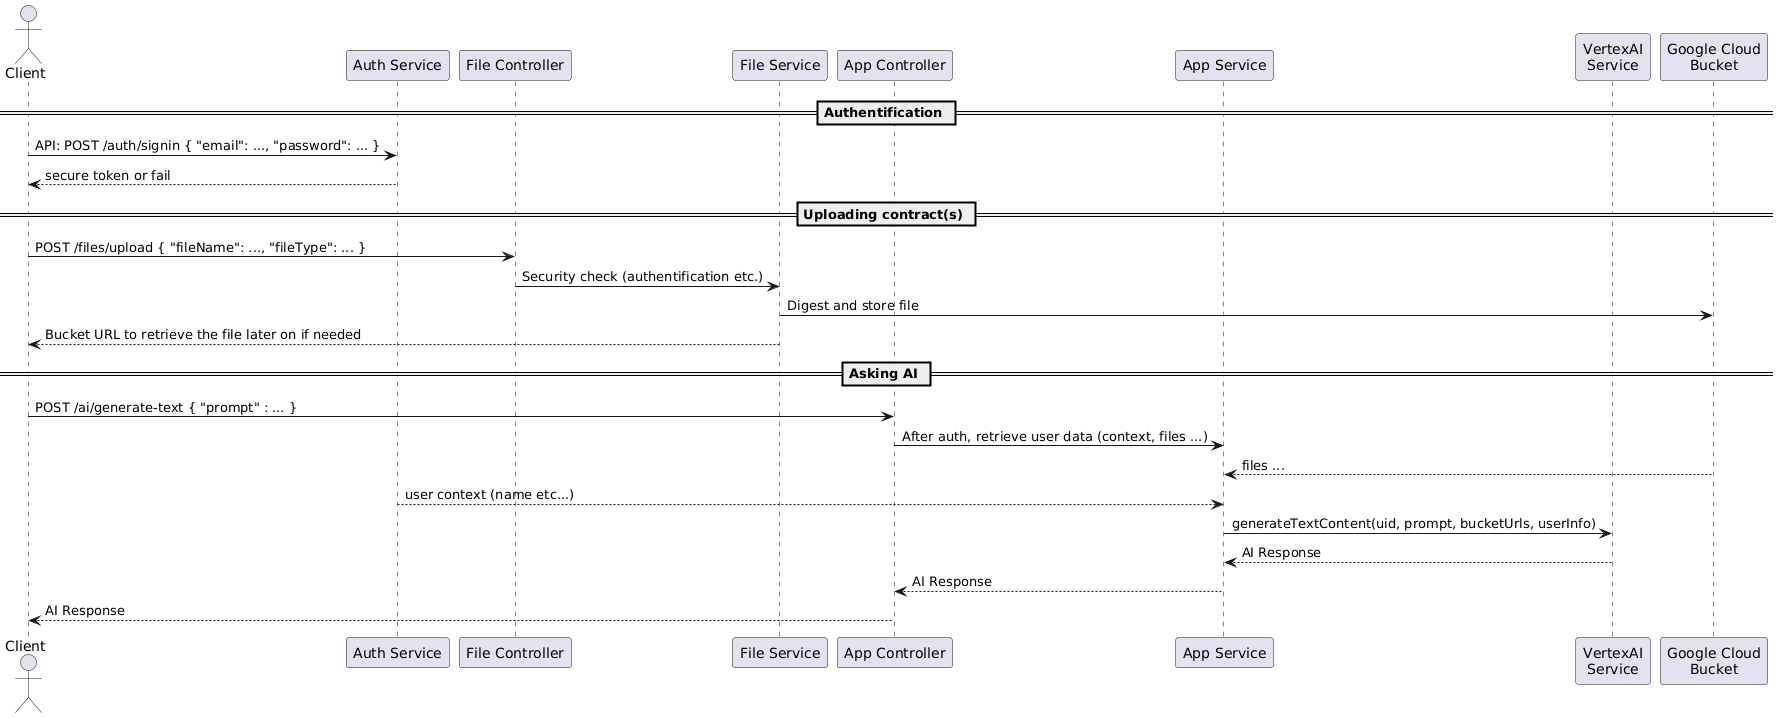
\includegraphics[width=\textheight]{nest/ai-sequence.png}
    \caption{Sequence diagram illustrating the AI processing flow}
    \label{fig:ai-sequence}
\end{sidewaysfigure}

\chapter{Microservice NestBackend}

\section{Overview}
\textbf{NestBackend} is the main backend service of the system. It integrates several key modules.

\section{Main Features}
\begin{itemize}
    \item \textbf{Authentication} using Firebase Auth
    \item \textbf{Firebase} in a GCP Cloud Storage bucket
    \item \textbf{VertexAI} with Gemini pro 1.5
    \item \textbf{Pub/Sub} messaging to communicate with DocAnalysis
    \item \textbf{Dashboard} for user to manage their documents
    \item \textbf{User} for user management
\end{itemize}

\section{Dependencies}

This section outlines the dependencies required for the backend service, categorized into service dependencies and development dependencies. Each dependency is listed with its purpose to provide clarity on its role within the project.
The backend service is built using the NestJS framework and integrates with various Google Cloud services, including Firebase and Vertex AI. The dependencies are managed using npm and are specified in the \texttt{package.json} file.

\subsection{Service Dependencies}

\begin{tabular}{>{\bfseries}l l}
\toprule
Package & Purpose \\
\midrule
@google-cloud/aiplatform & Vertex AI SDK for ML requests \\
@google-cloud/pubsub & Google Pub/Sub messaging system \\
@google-cloud/secret-manager & Secure storage and access to secrets \\
@google-cloud/vertexai & Vertex AI high-level client (simplified) \\
@nestjs/common & NestJS decorators and helpers \\
@nestjs/config & Environment configuration management \\
@nestjs/core & NestJS core engine \\
@nestjs/microservices & Microservice architecture support \\
@nestjs/platform-express & Express integration with NestJS \\
@nestjs/swagger & OpenAPI documentation generator \\
@types/multer & Type definitions for multer \\
class-transformer & DTO class serialization/deserialization \\
class-validator & DTO input validation \\
firebase-admin & Firebase Admin SDK (Auth, Firestore, GCS) \\
multer & Middleware for file uploads \\
nestjs-pino & Structured logging with Pino in NestJS \\
pino & High-performance JSON logger \\
reflect-metadata & Required for decorators/reflection \\
rxjs & Reactive programming and Observables \\
swagger-ui-express & Swagger UI middleware for Express \\
\bottomrule
\end{tabular}

\subsection{Dev Dependencies}

\begin{tabular}{>{\bfseries}l l}
\toprule
Package & Purpose \\
\midrule
@nestjs/cli & NestJS project scaffolding and commands \\
@nestjs/schematics & Code generation templates for NestJS \\
@nestjs/testing & Utilities for unit and integration tests \\
@types/express & Type definitions for Express.js \\
@types/jest & Type definitions for Jest \\
@types/node & Type definitions for Node.js \\
@types/supertest & Type definitions for Supertest \\
@typescript-eslint/eslint-plugin & ESLint rules for TypeScript \\
@typescript-eslint/parser & Parser to enable ESLint for TS \\
eslint & Linter for code quality \\
eslint-config-prettier & Disables rules that conflict with Prettier \\
eslint-plugin-prettier & Integrates Prettier into ESLint \\
jest & Testing framework \\
prettier & Code formatter \\
source-map-support & Stack trace source map translation \\
supertest & HTTP assertions for integration tests \\
ts-jest & Jest preprocessor for TypeScript \\
ts-loader & TypeScript loader for Webpack \\
ts-node & Run TypeScript files directly \\
tsconfig-paths & Support for path aliases in tsconfig \\
typescript & TypeScript compiler \\
\bottomrule
\end{tabular}
\section{User Module}

\subsection*{Overview}

The \textbf{UserModule} manages user-specific metadata and preferences that are not handled by Firebase Auth. It stores and retrieves information such as first name, last name, birthdate, and contact data using Firestore.

\subsection*{Responsibilities}

\begin{itemize}
    \item Create and update user profile information in Firestore.
    \item Retrieve authenticated user metadata (from Firebase Auth).
    \item Provide a minimal contact endpoint for support messages (placeholder).
\end{itemize}

\subsection*{Dependencies}

\begin{itemize}
    \item \texttt{Firestore} - Used to store extended user info.
    \item \texttt{AuthService} - Used to fetch Firebase Auth metadata (e.g., display name, email).
\end{itemize}

\subsection*{Key Service Methods}

\begin{itemize}
    \item \texttt{createUserInfo(uid, dto)}: Creates a Firestore document with full name and email pulled from Firebase Auth.
    \item \texttt{updateUserInfo(uid, dto)}: Updates the user info with merge semantics and a timestamp.
    \item \texttt{getUserInfo(uid)}: Returns user info from Firestore, or \texttt{null} if not found.
\end{itemize}

\subsection*{Exposed Routes}

\subsubsection*{POST /user/me}

\begin{tabular}{>{\bfseries}l l}
\toprule
Method & POST \\
Route & /user/me \\
Auth required & Yes \\
Status codes & 201 Created, 400 Bad Request, 401 Unauthorized \\
\bottomrule
\end{tabular}

\textbf{Description:} Creates the Firestore user profile based on the authenticated user's UID and metadata from Firebase Auth.

\vspace{1em}
\textbf{Payload Example:}
\begin{verbatim}
{
  "birthdate": "2000-01-01"
}
\end{verbatim}

\subsubsection*{PATCH /user/me}

\begin{tabular}{>{\bfseries}l l}
\toprule
Method & PATCH \\
Route & /user/me \\
Auth required & Yes \\
Status codes & 200 OK, 400 Bad Request, 401 Unauthorized \\
\bottomrule
\end{tabular}

\textbf{Description:} Updates user information in Firestore. Uses \texttt{merge: true} semantics to preserve existing fields.

\vspace{1em}
\textbf{Payload Example:}
\begin{verbatim}
{
  "firstname": "Jane",
  "lastname": "Smith",
  "email": "jane@example.com"
}
\end{verbatim}

\subsubsection*{POST /user/contact}

\begin{tabular}{>{\bfseries}l l}
\toprule
Method & POST \\
Route & /user/contact \\
Auth required & No \\
Status codes & 200 OK (placeholder) \\
\bottomrule
\end{tabular}

\textbf{Description:} Endpoint for users to contact admin/support. Currently a stub (to be implemented).

\vspace{1em}
\textbf{Payload Example:}
\begin{verbatim}
{
  "email": "user@example.com",
  "message": "I need help with..."
}
\end{verbatim}

\subsection*{Testing}

Unit tests validate:

\begin{itemize}
    \item Creation of user info from Firebase metadata.
    \item Updating user info with merge semantics.
    \item Retrieval of user data (existing and non-existing cases).
\end{itemize}

Mocks are used for:

\begin{itemize}
    \item \texttt{AuthService.getUserByUid()}
    \item Firestore collection, doc, set, and get operations
\end{itemize}

\section{Firebase Module}

\subsection*{Overview}

The \textbf{FirebaseModule} is a global dynamic module that initializes the Firebase Admin SDK and exposes key Firebase services throughout the application. It centralizes configuration and ensures consistent access to Firebase features like Firestore, Auth, and Cloud Storage.

\subsection*{Responsibilities}

\begin{itemize}
    \item Initialize Firebase Admin with default credentials.
    \item Provide access to:
        \begin{itemize}
            \item Firestore (NoSQL database)
            \item Firebase Authentication
            \item Cloud Storage bucket
        \end{itemize}
    \item Export these providers globally to be used by other modules (e.g., Auth, Files, Dashboard).
\end{itemize}

\subsection*{Dynamic Initialization}

\textbf{FirebaseModule.forRoot()} returns a \texttt{DynamicModule} configured with the following providers:

\begin{itemize}
    \item \textbf{FIREBASE\_APP} - Firebase application instance
    \item \textbf{FIRESTORE} - Firestore database instance
    \item \textbf{FIREBASE\_AUTH} - Firebase authentication handler
    \item \textbf{FIREBASE\_BUCKET} - Google Cloud Storage bucket handler
\end{itemize}

These tokens are injected via NestJS's dependency injection system.

\subsection*{Global Scope}

The module is marked with \texttt{@Global()} so it only needs to be imported once and is accessible throughout the entire application without re-importing in each feature module.

\subsection*{Testing}

A dedicated unit test verifies that:
\begin{itemize}
    \item All Firebase services are correctly provided via dependency tokens.
    \item The module exports all necessary services.
\end{itemize}

Mocked Firebase services are used in unit tests to avoid external dependency on Firebase during test execution.

\subsection*{Configuration}

\begin{itemize}
    \item \textbf{Project ID:} \texttt{contract-central-c710c}
    \item \textbf{Storage Bucket:} \texttt{contract-central-c710c.firebasestorage.app}
    \item \textbf{Credential:} Application Default Credential
\end{itemize}

\section{File Module}

\subsection*{Overview}

The \textbf{FileModule} manages all user file operations including upload, retrieval, deletion, and temporary storage. It integrates Google Cloud Storage via Firebase and uses Pub/Sub to notify other microservices of file-related events.

\subsection*{Responsibilities}

\begin{itemize}
    \item Upload and store user files under structured paths in GCS.
    \item Generate temporary signed URLs for accessing files.
    \item Delete specific or all files for a user.
    \item Notify other services of file upload and deletion via Pub/Sub.
\end{itemize}

\subsection*{Dependencies}

\begin{itemize}
    \item \texttt{@google-cloud/storage} - for GCS bucket access.
    \item \texttt{FirebaseModule} - to inject the GCS bucket.
    \item \texttt{PubSubService} - to publish \texttt{file-upload} and \texttt{file-delete} events.
\end{itemize}

\subsection*{Key Service Methods}

\begin{itemize}
    \item \texttt{uploadFile(uid, file, dto)} - Uploads a categorized file and emits Pub/Sub event.
    \item \texttt{getFileUrl(uid, fileName)} - Returns a temporary signed URL for a user file.
    \item \texttt{getUserFiles(uid)} - Lists all files uploaded by the user.
    \item \texttt{deleteFile(uid, fname, category)} - Deletes a file and emits a Pub/Sub event.
    \item \texttt{deleteAllUserFiles(uid)} - Deletes all user files and emits a single Pub/Sub event.
    \item \texttt{uploadTmpImage(uid, file, dto)} - Special-purpose method to upload temporary images.
    \item \texttt{deleteTempFile(fpath)} - Deletes a temporary file if it exists.
\end{itemize}

\subsection*{Exposed Routes}

\subsubsection*{POST /files/upload}

\begin{tabular}{>{\bfseries}l l}
\toprule
Method & POST \\
Route & /files/upload \\
Auth required & Yes \\
Consumes & multipart/form-data \\
\bottomrule
\end{tabular}

\vspace{1em}
\textbf{Form fields:}
\begin{itemize}
    \item \texttt{file}: PDF file to upload
    \item \texttt{category}: required category label (e.g., \texttt{HEALTH}, \texttt{EMPLOYMENT})
\end{itemize}

\subsubsection*{GET /files/:fileName}

Returns a temporary signed URL for the requested file.

\subsubsection*{GET /files}

Returns a list of all files uploaded by the authenticated user.

\subsubsection*{DELETE /files/:category/:fileName}

Deletes a specific file in a category and emits a \texttt{file-delete} event.

\subsubsection*{DELETE /files}

Deletes all files for the user and emits a single \texttt{file-delete} event.

\subsection*{Error Handling}

\begin{itemize}
    \item \textbf{400 Bad Request} - Invalid or missing category.
    \item \textbf{404 Not Found} - Requested file does not exist.
    \item \textbf{500 Internal Server Error} - Upload/delete/signing failures.
\end{itemize}

\subsection*{Testing}

Unit tests validate:

\begin{itemize}
    \item File upload with event publishing.
    \item Temporary signed URL generation.
    \item Accurate file listing.
    \item Conditional deletion (specific or all files).
    \item Handling of missing files and errors.
\end{itemize}

Mocks are used for:

\begin{itemize}
    \item GCS Bucket and File objects.
    \item Pub/Sub message publishing.
\end{itemize}

\section{VertexAI Module}

\subsection*{Overview}

The \textbf{VertexAI Module} integrates the Google Cloud Vertex AI API into the backend using the \texttt{@google-cloud/vertexai} client. It handles AI-driven reasoning and recommendation tasks by interacting with Gemini 1.5 Pro.

\subsection*{Responsibilities}

\begin{itemize}
    \item Load a generative model (Gemini 1.5 Pro) via the Vertex AI SDK.
    \item Process user prompts and file references (PDF, images).
    \item Generate structured reasoning and actionable recommendations.
    \item Log AI interactions to Firestore for traceability.
\end{itemize}

\subsection*{Workflow Summary}

The method \texttt{generateTextContent} executes two chained LLM calls:

\begin{enumerate}
    \item \textbf{Structured reasoning generation} based on:
    \begin{itemize}
        \item User metadata (\texttt{firstname}, \texttt{lastname}, etc.)
        \item Attached files from Firebase Storage
        \item Custom domain-specific reasoning prompt
    \end{itemize}
    \item \textbf{Final decision generation} based on the AI's reasoning output.
\end{enumerate}

Results are logged in Firestore under the \texttt{logs/\{uid\}/ai\_interactions} collection with full metadata.

\subsection*{Prompt Logic}

\begin{itemize}
    \item Prompts are composed dynamically using the user's identity and structured business rules.
    \item \textbf{Reasoning Prompt:} guides the model to extract risk analysis and contract redundancies.
    \item \textbf{Final Decision Prompt:} asks the model to produce an actionable summary.
    \item All file attachments are referenced using GCS URIs (e.g., \texttt{gs://bucket/path}).
\end{itemize}

\subsection*{Key Method: \texttt{generateTextContent}}

\begin{itemize}
    \item \textbf{Inputs:} user ID, prompt string, list of Firebase Storage URLs, user metadata.
    \item \textbf{Output:} response object from Vertex AI's LLM (Gemini 1.5 Pro).
    \item \textbf{Side-effects:}
    \begin{itemize}
        \item AI interaction logs written to Firestore.
        \item Token usage, model version, and response IDs tracked.
    \end{itemize}
\end{itemize}

\subsection*{Firestore Logging Structure}

Each interaction creates or updates a Firestore document with:

\begin{itemize}
    \item \texttt{prompt}, \texttt{reasoning}, \texttt{finalDecision}
    \item \texttt{vertexResponse} and \texttt{finalVertexResponse} metadata
    \item \texttt{createdAt}, \texttt{deletedAt}
\end{itemize}

\subsection*{Error Handling}

\begin{itemize}
    \item If reasoning or decision generation fails, the error is logged and rethrown.
    \item GCS URI generation fallback uses MIME type detection to support different file types.
\end{itemize}

\subsection*{Testing}

Unit tests validate:

\begin{itemize}
    \item Proper generation of both reasoning and final decision via mocked LLM.
    \item Firestore logs are created and updated accordingly.
    \item Token usage, model version, and response IDs are extracted correctly.
\end{itemize}

Mocks are used for:

\begin{itemize}
    \item VertexAI client and model generation responses.
    \item Firestore document creation and update.
\end{itemize}

\section{Dashboard Module}

\subsection*{Overview}

The \textbf{Dashboard} module provides a synthetic view of a user's activity and data. It aggregates file statistics and coverage request history from Firestore and returns a structured dashboard summary.

\subsection*{Responsibilities}

\begin{itemize}
    \item Aggregate file statistics per user from Cloud Storage.
    \item Count and classify AI coverage requests (pending / completed).
    \item Return a structured summary to the frontend.
\end{itemize}

\subsection*{Dependencies}

\begin{itemize}
    \item \texttt{FileService} - for retrieving user files from storage.
    \item \texttt{Firestore} - for querying the \texttt{coverage\_requests} collection.
    \item \texttt{@nestjs/common} - for DI and controller structure.
\end{itemize}

\subsection*{Main Service Method}

\begin{itemize}
    \item \textbf{buildDashboard(uid: string)}: builds and returns a \texttt{DashboardDto} object containing:
    \begin{itemize}
        \item Total number of user files
        \item Breakdown of files by category
        \item Coverage requests (pending and completed)
        \item Recent request history (max 20)
    \end{itemize}
\end{itemize}

\subsection*{Resilience Handling}

If the required Firestore index is missing, a partial dashboard is returned with empty coverage history. This ensures continued availability even when Firestore is misconfigured.

\subsection*{Exposed Route}

\subsubsection*{GET /dashboard}

\begin{tabular}{>{\bfseries}l l}
\toprule
Method & GET \\
Route & /dashboard \\
Auth required & Yes (via Firebase ID token) \\
Status codes & 200 OK, 500 Internal Server Error \\
\bottomrule
\end{tabular}

\vspace{1em}
\textbf{Headers:}
\begin{verbatim}
Authorization: Bearer <ID_TOKEN>
\end{verbatim}

\vspace{1em}
\textbf{Success Response:}
\begin{verbatim}
Status: 200 OK
{
  "totalFiles": 3,
  "filesByCategory": {
    "health": 1,
    "employment": 2
  },
  "pendingCoverageRequests": 1,
  "completedCoverageRequests": 4,
  "coverageHistory": [
    {
      "requestId": "abc123",
      "prompt": "What is my health coverage?",
      "status": "done",
      "response": "...",
      "updatedAt": 1716170000000
    }
  ]
}
\end{verbatim}

\vspace{1em}
\textbf{Error Responses:}
\begin{itemize}
    \item \textbf{500 Internal Server Error} - Firestore failure or exception.
\end{itemize}

\section{PubSub Module}

\subsection*{Overview}

The \textbf{PubSubModule} encapsulates the Google Cloud Pub/Sub integration used by the application to handle asynchronous communication between microservices. It publishes and subscribes to various event topics related to files and AI coverage analysis.

\subsection*{Responsibilities}

\begin{itemize}
    \item Publish events to specific Pub/Sub topics.
    \item Subscribe to the \texttt{coverage-response-sub} subscription.
    \item Update Firestore with AI coverage results upon message reception.
\end{itemize}

\subsection*{Topics Used}

\begin{itemize}
    \item \textbf{coverage-query} - Trigger coverage analysis requests.
    \item \textbf{coverage-response} - Receives responses from the AI service.
    \item \textbf{file-upload} - Event triggered when a file is uploaded.
    \item \textbf{file-delete} - Event triggered when a file is deleted.
\end{itemize}

\subsection*{Key Methods}

\begin{itemize}
    \item \texttt{publishMessage(topicName: string, data: object)} \\
    Publishes a JSON-encoded message to the specified Pub/Sub topic.

    \item \texttt{subscribeToCoverageResponse()} \\
    Subscribes to \texttt{coverage-response-sub} and processes AI results to update the Firestore \texttt{coverage\_requests} collection.
\end{itemize}

\subsection*{Error Handling}

If a received message is missing expected fields (\texttt{request\_id}, \texttt{user\_uuid}, or \texttt{response}), the message is rejected with \texttt{nack()}. Other exceptions are logged and also result in a negative acknowledgment.

\subsection*{Lifecycle Hook}

The service implements \texttt{OnModuleInit} and only subscribes to incoming Pub/Sub messages if the environment is not \texttt{"test"}. This allows for isolated unit testing without background consumers.

\subsection*{Testing}

Unit tests verify:
\begin{itemize}
    \item That messages are published correctly with expected parameters.
    \item That the \texttt{subscribeToCoverageResponse} method is invoked on module initialization (except in test mode).
    \item That Firestore is updated when a message is handled successfully.
\end{itemize}

Mocks are used for:
\begin{itemize}
    \item Pub/Sub client, topics and subscriptions.
    \item Firestore client and document operations.
\end{itemize}

\section{VertexAI Module}

\subsection*{Overview}

The \textbf{VertexAI Module} integrates the Google Cloud Vertex AI API into the backend using the \texttt{@google-cloud/vertexai} client. It handles AI-driven reasoning and recommendation tasks by interacting with Gemini 1.5 Pro.

\subsection*{Responsibilities}

\begin{itemize}
    \item Load a generative model (Gemini 1.5 Pro) via the Vertex AI SDK.
    \item Process user prompts and file references (PDF, images).
    \item Generate structured reasoning and actionable recommendations.
    \item Log AI interactions to Firestore for traceability.
\end{itemize}

\subsection*{Workflow Summary}

The method \texttt{generateTextContent} executes two chained LLM calls:

\begin{enumerate}
    \item \textbf{Structured reasoning generation} based on:
    \begin{itemize}
        \item User metadata (\texttt{firstname}, \texttt{lastname}, etc.)
        \item Attached files from Firebase Storage
        \item Custom domain-specific reasoning prompt
    \end{itemize}
    \item \textbf{Final decision generation} based on the AI's reasoning output.
\end{enumerate}

Results are logged in Firestore under the \texttt{logs/\{uid\}/ai\_interactions} collection with full metadata.

\subsection*{Prompt Logic}

\begin{itemize}
    \item Prompts are composed dynamically using the user's identity and structured business rules.
    \item \textbf{Reasoning Prompt:} guides the model to extract risk analysis and contract redundancies.
    \item \textbf{Final Decision Prompt:} asks the model to produce an actionable summary.
    \item All file attachments are referenced using GCS URIs (e.g., \texttt{gs://bucket/path}).
\end{itemize}

\subsection*{Key Method: \texttt{generateTextContent}}

\begin{itemize}
    \item \textbf{Inputs:} user ID, prompt string, list of Firebase Storage URLs, user metadata.
    \item \textbf{Output:} response object from Vertex AI's LLM (Gemini 1.5 Pro).
    \item \textbf{Side-effects:}
    \begin{itemize}
        \item AI interaction logs written to Firestore.
        \item Token usage, model version, and response IDs tracked.
    \end{itemize}
\end{itemize}

\subsection*{Firestore Logging Structure}

Each interaction creates or updates a Firestore document with:

\begin{itemize}
    \item \texttt{prompt}, \texttt{reasoning}, \texttt{finalDecision}
    \item \texttt{vertexResponse} and \texttt{finalVertexResponse} metadata
    \item \texttt{createdAt}, \texttt{deletedAt}
\end{itemize}

\subsection*{Error Handling}

\begin{itemize}
    \item If reasoning or decision generation fails, the error is logged and rethrown.
    \item GCS URI generation fallback uses MIME type detection to support different file types.
\end{itemize}

\subsection*{Testing}

Unit tests validate:

\begin{itemize}
    \item Proper generation of both reasoning and final decision via mocked LLM.
    \item Firestore logs are created and updated accordingly.
    \item Token usage, model version, and response IDs are extracted correctly.
\end{itemize}

Mocks are used for:

\begin{itemize}
    \item VertexAI client and model generation responses.
    \item Firestore document creation and update.
\end{itemize}

\section{Auth Module}

\subsection*{Overview}

The \textbf{Auth} module handles user creation and authentication token validation using the Firebase Admin SDK. It provides a simple REST interface to register new users and verify existing sessions.

\subsection*{Responsibilities}

\begin{itemize}
    \item Creating new users via Firebase.
    \item Verifying ID tokens for secure API access.
    \item Fetching user information by UID.
\end{itemize}

\subsection*{Dependencies}

\begin{itemize}
    \item \texttt{firebase-admin} - for user management and token verification.
    \item \texttt{@nestjs/common} - core NestJS features.
    \item \texttt{class-validator} - request payload validation (via DTO).
\end{itemize}

\subsection*{Main Service Methods}

\begin{itemize}
    \item \textbf{create(dto: CreateUserDto)}: registers a user in Firebase.
    \item \textbf{checkToken(token: string)}: verifies a Firebase ID token.
    \item \textbf{getUserByUid(uid: string)}: fetches user data from Firebase.
\end{itemize}

\subsection*{Testing}

Unit tests are implemented with Jest and cover:
\begin{itemize}
    \item User creation with full name.
    \item Token verification.
    \item User retrieval by UID.
\end{itemize}

\subsection*{Exposed Route}

\subsubsection*{POST /auth/signin}

\begin{tabular}{>{\bfseries}l l}
\toprule
Method & POST \\
Route & /auth/signin \\
Auth required & No \\
Status codes & 201 Created, 400 Bad Request, 500 Internal Server Error \\
\bottomrule
\end{tabular}

\vspace{1em}
\textbf{Request Body:}
\begin{verbatim}
{
  "email": "john@example.com",
  "password": "securePass123",
  "firstname": "John",
  "lastname": "Doe"
}
\end{verbatim}

\vspace{1em}
\textbf{Success Response:}
\begin{verbatim}
Status: 201 Created
{
  "statusCode": 201,
  "message": "User created",
  "data": {
    "uid": "user123",
    ...
  }
}
\end{verbatim}

\vspace{1em}
\textbf{Error Responses:}
\begin{itemize}
    \item \textbf{400 Bad Request} - missing or invalid fields.
    \item \textbf{500 Internal Server Error} - Firebase failure or exception.
\end{itemize}

\subsection*{AI Interaction Sequence}

\begin{sidewaysfigure}
    \centering
    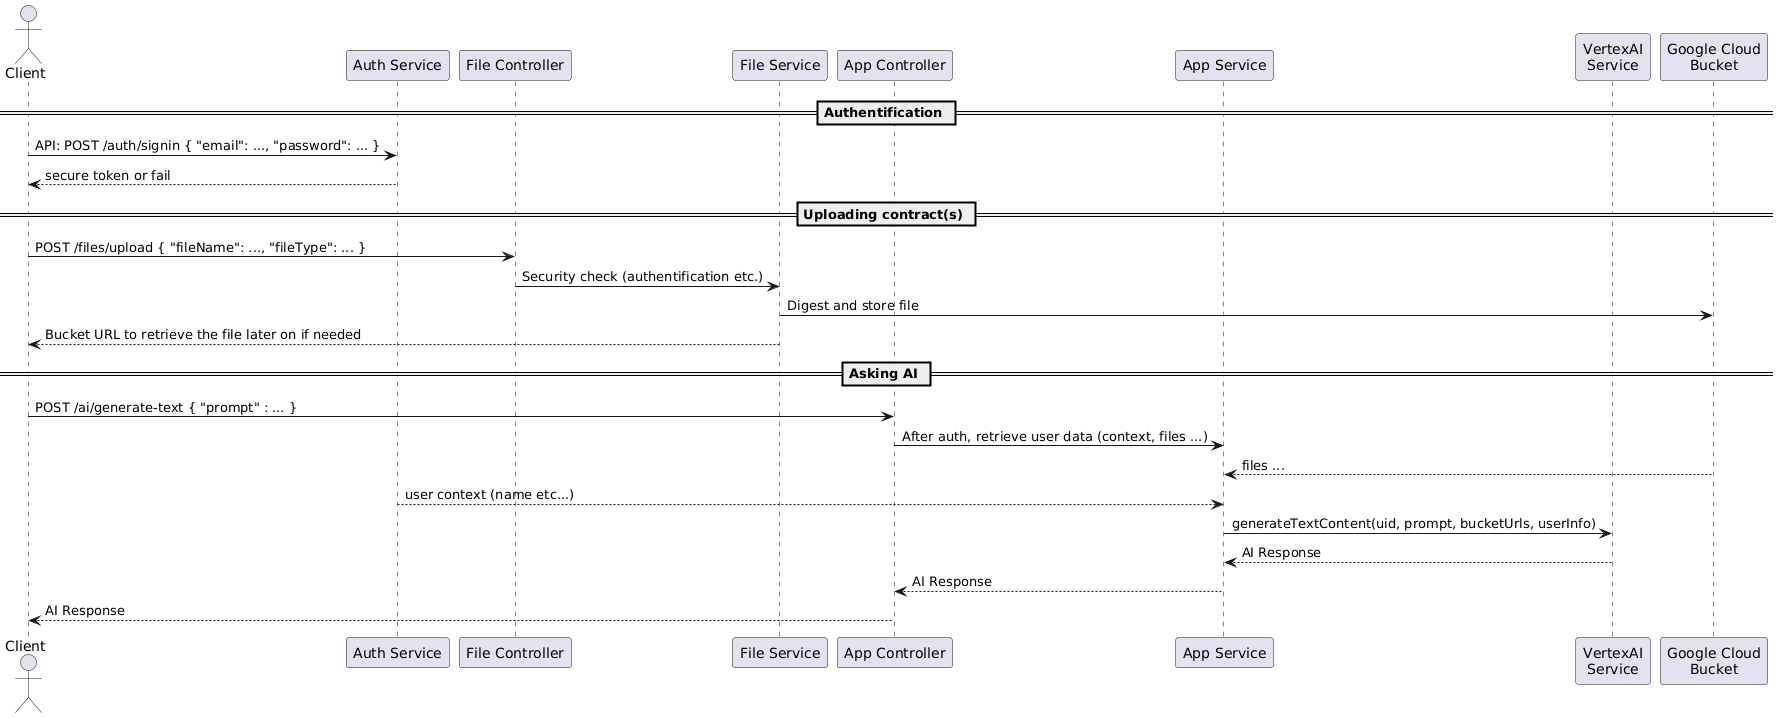
\includegraphics[width=\textheight]{nest/ai-sequence.png}
    \caption{Sequence diagram illustrating the AI processing flow}
    \label{fig:ai-sequence}
\end{sidewaysfigure}


\chapter*{Conclusion}
\addcontentsline{toc}{chapter}{Conclusion}

This documentation presented the architecture, technical design, and implementation details of the Contract Central project. The system combines a mobile/web frontend built with Flutter, a scalable backend hosted on Google Cloud, and AI-driven document analysis using Gemini and ChromaDB.

Each component was developed as an independent microservice to promote modularity and ease of maintenance. The CI/CD pipeline, based on GitHub Actions, enables automated testing and deployment to Cloud Run.

The frontend was designed to offer a smooth, cross-platform user experience, while the backend ensures security and scalability through asynchronous messaging and vector-based search.

This project highlights the power of combining cloud infrastructure, AI, and cross-platform development to deliver a real-world solution for contract management.


\end{document}
